\documentclass{report}

\usepackage{amsmath, array, bm, enumerate, tikz, pgfplots, sfmath, multicol, hyperref, afterpage}
\pgfplotsset{compat = 1.16}
\usepackage[margin = 0.5in]{geometry}
\raggedright
\renewcommand{\familydefault}{\sfdefault}
\newcounter{Review}
\usetikzlibrary{fadings}

\begin{document}
\begin{titlepage}
\DeclareFixedFont{\titlefont}{T1}{ppl}{b}{}{0.7in}
\DeclareFixedFont{\subtitlefont}{T1}{ppl}{b}{}{0.4in}
\afterpage{\restoregeometry}
\newgeometry{left=1in, right=1in,top=1in, bottom=0in}
\definecolor{stainedglassblue}{HTML}{2E37FE}
\pagecolor{stainedglassblue}\afterpage{\nopagecolor}

\thispagestyle{empty}
\begin{center}
\color{white}{
\titlefont Honors PreCalculus	\vfill
\scalebox{3}{${\displaystyle \sum_{\text{Algebra}}^{\text{Calculus}}  } $}
\vfill 
\subtitlefont Review}
\end{center}
\vfill
\end{titlepage}


\tableofcontents
\chapter{Basic Set Theory and Interval Notation}

You are given either interval notation, set-builder notation, or a graph. Write each of the following in its other 2 forms. 
\begin{enumerate}
\setlength\itemsep{10pt}
    \item $(-5, 8]$
    \item $\{x|x \leq 1\}$
    \item
    \raisebox{-8pt}{
    \begin{tikzpicture}
    \draw [->] (-2,0) node [below, yshift=-4pt] {$-3$} -- (2,0);
    \draw [fill=black] (-2,0) circle [radius=2.5pt];
    \end{tikzpicture}}
    \item $\{x | x \neq 4, 11\}$
    \item
    \raisebox{-8pt}{
    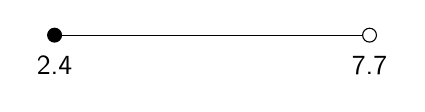
\begin{tikzpicture}
        \draw (-2,0) node [below, yshift=-4pt] {$2.4$} -- (2,0) node [below, yshift=-4pt] {$7.7$};
        \draw [fill=black] (-2,0) circle [radius=2.5pt];
        \draw [fill=white] (2,0) circle [radius=2.5pt];
    \end{tikzpicture}}
    \item $(9, \infty)$
\setcounter{Review}{\value{enumi}}
\end{enumerate}

Write each using interval notation and graph on a number line.
\begin{enumerate}
\setcounter{enumi}{\value{Review}}
\item $\{x | x \geq 2\}$
\item $\{x |x < -8\}$
\item $\{x |x \neq 3\}$
\item $\{x | x \neq -2, 5\}$
\setcounter{Review}{\value{enumi}}
\end{enumerate}

You are given the graph of an interval. Write the interval and set-builder notation for it.
\begin{enumerate}
\setcounter{enumi}{\value{Review}}
\item \raisebox{-10pt}{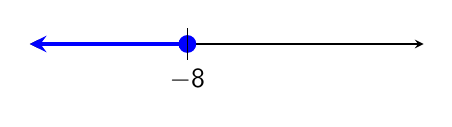
\begin{tikzpicture}[>=stealth]
    \draw[<->] (-2.5,0) -- (2.5,0);
    \filldraw[color=blue] (-0.5,0) circle [radius=3pt];
    \draw (-0.5,0.2) -- (-0.5,-0.2) node [below] {$-8$};
    \draw[color=blue,ultra thick, ->] (-0.5,0) -- (-2.5,0);
    \end{tikzpicture}}

\item \raisebox{-10pt}{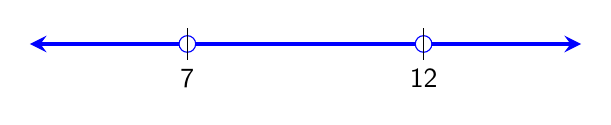
\begin{tikzpicture}[>=stealth]
    \draw[<->, color=blue, ultra thick] (-3.5,0) -- (3.5,0);
    \draw[color=blue, fill=white] (-1.5,0) circle [radius=3pt];
    \draw[color=blue, fill=white] (1.5,0) circle [radius=3pt];
    \draw (-1.5,0.2) -- (-1.5,-0.2) node [below] {$7$};
    \draw (1.5,0.2) -- (1.5,-0.2) node [below] {$12$};
    \end{tikzpicture}}
    
\item \raisebox{-10pt}{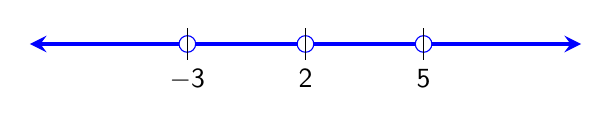
\begin{tikzpicture}[>=stealth]
    \draw[<->, color=blue, ultra thick] (-3.5,0) -- (3.5,0);
    \draw[color=blue, fill=white] (-1.5,0) circle [radius=3pt];
    \draw[color=blue, fill=white] (1.5,0) circle [radius=3pt];
    \draw[color=blue, fill=white] (0,0) circle [radius=3pt];
    \draw (-1.5,0.2) -- (-1.5,-0.2) node [below] {$-3$};
    \draw (0,0.2) -- (0,-0.2) node [below] {$2$};
    \draw (1.5,0.2) -- (1.5,-0.2) node [below] {$5$};
    \end{tikzpicture}}
\end{enumerate}

\newpage

\section{Answer Key}

\begin{enumerate}
\setlength\itemsep{10pt}
	\item $\{x | -5 < x \leq 8\}$	\newline\\
	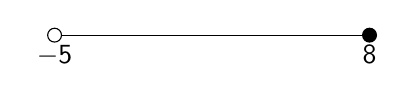
\begin{tikzpicture}
	\draw (-2,0) node [below] {$-5$} -- (2,0) node [below] {$8$};
	\draw [fill=white] (-2,0) circle [radius = 2.5pt];
	\draw [fill=black] (2,0) circle [radius = 2.5pt];
	\end{tikzpicture}
	
	\item $(-\infty, 1]$ \newline\\
	\begin{tikzpicture}
	\draw [<-] (-2,0) -- (2,0) node [below] {1};
	\draw [fill=black] (2,0) circle [radius=2.5pt];
	\end{tikzpicture}
	
	\item $[-3, \infty)$ \quad $\{x | x \geq -3 \}$
	
	\item $(-\infty, 4) \cup (4, 11) \cup (11, \infty)$ \newline\\
	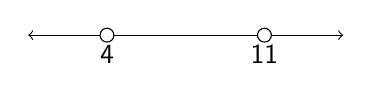
\begin{tikzpicture}
	\draw[<->] (-2,0) -- (2,0);
	\draw[fill=white] (-1,0) circle [radius=2.5pt];
	\draw[fill=white] (1,0) circle [radius=2.5pt];
	\node at (-1,0) [below] {4};
	\node at (1,0) [below] {11};
	\end{tikzpicture}
	
	\item $[2.4, 7.7)$ \quad $\{x | 2.4 \leq x < 7.7\}$
	
	\item $\{x | x > 9\}$ \newline\\
	\begin{tikzpicture}
	\draw[->] (-2,0) -- (2,0);
	\draw[fill=white] (-2,0) circle [radius=2.5pt];
	\node at (-2,0) [below] {9};
	\end{tikzpicture}

	\item $[2, \infty)$ \newline\\
	\begin{tikzpicture}
	\draw[->] (-2,0) -- (2,0);
	\draw[fill=black] (-2,0) circle [radius=2.5pt];
	\node at (-2,0) [below] {2};
	\end{tikzpicture}
	
	\item $(-\infty, -8)$ \newline\\
	\begin{tikzpicture}
	\draw[<-] (-2,0) -- (2,0);
	\draw[fill=white] (2,0) circle [radius=2.5pt];
	\node at (2,0) [below] {$-8$};
	\end{tikzpicture}
	
	\item $(-\infty, 3) \cup (3, \infty)$ \newline\\
	\begin{tikzpicture}
	\draw[<->] (-2,0) -- (2,0);
	\draw[fill=white] (0,0) circle [radius=2.5pt];
	\node at (0,0) [below] {3};
	\end{tikzpicture}
	
	\item $(\infty, -2) \cup (-2,5) \cup (5,\infty)$ \newline\\
	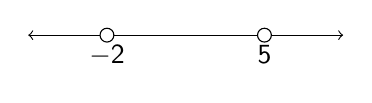
\begin{tikzpicture}
	\draw[<->] (-2,0) -- (2,0);
	\draw[fill=white] (-1,0) circle [radius=2.5pt];
	\draw[fill=white] (1,0) circle [radius=2.5pt];
	\node at (-1,0) [below] {$-2$};
	\node at (1,0) [below] {5};	
	\end{tikzpicture}
	
	\item $(-\infty, -8]$ \quad $\{ x | x \leq -8 \}$
    \item $(-\infty,7) \cup (7,12) \cup (12, \infty)$ \quad $\{ x | x \neq 7, 12 \}$
    \item $(-\infty,-3) \cup (-3,2) \cup (2, 5) \cup (5, \infty)$ \quad $\{ x | x \neq -3, 2, 5 \}$
\end{enumerate}



\chapter{Functions and Their Graphs}

\section{Evaluating Functions}

The essence of functions can be summarized as follows:

\begin{enumerate}
    \item Take an input
    \item Process it according to how the function is defined
    \item Return a result as output
\end{enumerate}

We can give functions numerical or algebraic values. \\[18pt]

Regardless of what type of input we give a function, you will need to remember your {\color{violet}\textbf{order of operations}} when processing that input. For each step in the order of operations, perform each step completely before moving on to the next step.

\begin{enumerate}
    \item Simplify any expressions inside parentheses.
    \item Evaluate any exponential expressions
    \item Perform any multiplication or division \emph{in the order in which they appear}.
    \item Perform any addition or subtraction \emph{in the order in which they appear}.
\end{enumerate}

\vspace{18pt}

\begin{example}
Given $f(x) = -6x^2 - 5x + 2$, evaluate each of the following.
\begin{multicols}{3}
\begin{enumerate}[(a)]
    \item $f(7)$
    \item $f(3x)$
    \item $f(5x - 6)$
\end{enumerate}
\end{multicols}
\end{example}

\begin{solution}
$f(x)$'s whole purpose is to perform the following process:

\begin{enumerate}
    \item Square the input you give it
    \item Multiply that result by $-6$
    \item Multiply the input by 5 and subtract that from the previous step
    \item Add 2 to the result from the previous step
\end{enumerate}

(a)  $f(7)$

\begin{align*}
    f(7) &= -6(7)^2 - 5(7) + 2 \\
    &= -6(49) - 5(7) + 2 \qquad 7^2 = 49 \\
    &= -294 - 5(7) + 2 \qquad -6(49) = -294 \\
    &= -294 - 35 + 2 \qquad 5(7) = 35 \\
    &= -329 + 2 \qquad -294-35 = -329 \\
    &= -327
\end{align*}

(b)  $f(3x)$

\begin{align*}
    f(3x) &= -6(3x)^2 - 5(3x) + 2 \\
    &= -6(9x^2) - 5(3x) + 2 \qquad (3x)^2 = 9x^2 \\
    &= -54x^2 - 5(3x) + 2 \qquad -6(9x^2) = -54x^2 \\
    &= -54x^2 - 15x + 2 \qquad 5(3x) = 15x \\
    &= -54x^2 - 15x + 2 \qquad \text{no like terms to combine} 
\end{align*}

(c)  $f(5x-6)$

\begin{align*}
    f(5x-6) &= -6(5x-6)^2 - 5(5x-6) + 2 \\ 
    &= -6(25x^2 - 60x + 36) - 5(5x-6) + 2 \qquad (5x-6)^2 = 25x^2 - 60x + 36 \\
    &= -150x^2 + 360x - 216 - 5(5x-6) + 2 \qquad \text{distribute the $-6$} \\
    &= -150x^2 + 360x - 216 - 25x + 30 + 2 \qquad \text{distribute the $-5$} \\
    &= -150x^2 + 335x - 184 \qquad \text{combine like terms}
\end{align*}
\end{solution}

\section{Exercises}

\subsection*{Evaluating Functions}

Given $f(x) = -3x^2 + 4x$ and $g(x) = \frac{1}{x}-5$, evaluate each.
\begin{multicols}{3}
\begin{enumerate}
	\item $f(5)$
	\item $f(-2)$
	\item $f(0)$
\end{enumerate}	\setcounter{Review}{\value{enumi}}
\end{multicols}
\begin{multicols}{3}
\begin{enumerate}	\setcounter{enumi}{\value{Review}}
	\item $g(1)$
	\item $g(-5)$
	\item $g(1/4)$
\end{enumerate}	\setcounter{Review}{\value{enumi}}
\end{multicols}
\begin{multicols}{3}
\begin{enumerate}	\setcounter{enumi}{\value{Review}}
	\item $f(-x)$
	\item $g(-x)$
	\item $f(2x)$
\end{enumerate}	\setcounter{Review}{\value{enumi}}
\end{multicols}
\begin{multicols}{3}
\begin{enumerate}	\setcounter{enumi}{\value{Review}}
	\item $g(2x)$
	\item $f(x-3)$
	\item $g(x-3)$
\end{enumerate}	\setcounter{Review}{\value{enumi}}
\end{multicols}
\begin{multicols}{3}
\begin{enumerate}	\setcounter{enumi}{\value{Review}}
	\item $f\left(\frac{1}{3}x\right)$
	\item $g\left(\frac{1}{3}x\right)$
	\item $f(2x+1)$
\end{enumerate}	\setcounter{Review}{\value{enumi}}
\end{multicols}
\begin{multicols}{3}
\begin{enumerate}	\setcounter{enumi}{\value{Review}}
	\item $g(2x+1)$
	\item $f(-x+7)$
	\item $g(-x+7)$
\end{enumerate}
\end{multicols}

\subsection*{Domain of Functions}

Find the domain of each write your answers in interval notation.
\begin{multicols}{3}
\begin{enumerate}
	\item $f(x) = -8x^2 - 7x + 1$
	\item $g(x) = \sqrt{5x+12}-2$
	\item $h(x) = \frac{x+2}{9x-7}$
\end{enumerate}	\setcounter{Review}{\value{enumi}}
\end{multicols}
\begin{multicols}{3}
\begin{enumerate}	\setcounter{enumi}{\value{Review}}
	\item $f(x) = -5x + 4$
	\item $f(x) = x^2 + 2$
	\item $f(x) = \frac{2x+1}{3x-5}$
\end{enumerate}	\setcounter{Review}{\value{enumi}}
\end{multicols}
\begin{multicols}{3}
\begin{enumerate}	\setcounter{enumi}{\value{Review}}
	\item $f(x) = \sqrt{3x-12}$
	\item $f(x) = \frac{x}{x^2-16}$
	\item $f(x) = \frac{x+4}{x^3-4x}$
\end{enumerate}	\setcounter{Review}{\value{enumi}}
\end{multicols}
\begin{multicols}{3}
\begin{enumerate}	\setcounter{enumi}{\value{Review}}
	\item $f(x) = \frac{x}{\sqrt{x-4}}$
	\item $f(x) = \frac{x^2+1}{2x^2+8}$
	\item $f(x) = -\frac{x+7}{x^2-5x-6}$
\end{enumerate}	\setcounter{Review}{\value{enumi}}
\end{multicols}
\begin{multicols}{3}
\begin{enumerate}	\setcounter{enumi}{\value{Review}}
	\item $g(x) = \sqrt{2x+3}$
	\item $h(x) = \sqrt[3]{2x+3}$
	\item $f(x) = -\frac{7x-10}{x^2+3x+2}$
\end{enumerate}	\setcounter{Review}{\value{enumi}}
\end{multicols}
\begin{multicols}{3}
\begin{enumerate}	\setcounter{enumi}{\value{Review}}
	\item $g(x) = \sqrt{-9x+8}$
	\item $h(x) = -\sqrt[3]{4x+1}$
	\item $f(x) = \sqrt[3]{8x+1}$
\end{enumerate}	\setcounter{Review}{\value{enumi}}
\end{multicols}
\begin{multicols}{3}
\begin{enumerate}	\setcounter{enumi}{\value{Review}}
	\item $g(x) = \frac{x^2-1}{\sqrt{x+3}}$
	\item $h(x) = \frac{3}{9 + \frac{4}{x+7}}$
	\item $f(x) = \frac{x+1}{\sqrt{10x+8}}$
\end{enumerate}	\setcounter{Review}{\value{enumi}}
\end{multicols}
\begin{multicols}{3}
\begin{enumerate}	\setcounter{enumi}{\value{Review}}
	\item $g(x) = \frac{5}{1+\frac{3}{x+2}}$
	\item $i(x) = \frac{7}{3-\frac{4}{x+1}}$
	\item $n(x) = \frac{7x+14}{\sqrt{2x-1}}$
\end{enumerate}	\setcounter{Review}{\value{enumi}}
\end{multicols}
\begin{multicols}{3}
\begin{enumerate}	\setcounter{enumi}{\value{Review}}
	\item $a(x) = \dfrac{\frac{x}{x-2}}{{\frac{3}{x-2}+6}}$
	\item $d(x) = \frac{7x-5}{\sqrt[3]{5x+2}}$
\end{enumerate}
\end{multicols}



\newpage

\section{Answer Key}

\subsection*{Evaluating Functions}

\begin{multicols}{3}
\begin{enumerate}
	\item $-55$
	\item $-20$
	\item 0
\end{enumerate}	\setcounter{Review}{\value{enumi}}
\end{multicols}
\begin{multicols}{3}
\begin{enumerate}	\setcounter{enumi}{\value{Review}}
	\item $-4$
	\item $-5.2$
	\item $-1$
\end{enumerate}	\setcounter{Review}{\value{enumi}}
\end{multicols}
\begin{multicols}{3}
\begin{enumerate}	\setcounter{enumi}{\value{Review}}
	\item $-3x^2 - 4x$
	\item $-\frac{1}{x}-5 = \frac{-1-5x}{x}$
	\item $-12x^2 + 8x$
\end{enumerate}	\setcounter{Review}{\value{enumi}}
\end{multicols}
\begin{multicols}{3}
\begin{enumerate}	\setcounter{enumi}{\value{Review}}
	\item $\frac{1-10x}{2x}$
	\item $-3x^2 + 22x - 39$
	\item $\frac{16-5x}{x-3}$
\end{enumerate}	\setcounter{Review}{\value{enumi}}
\end{multicols}
\begin{multicols}{3}
\begin{enumerate}	\setcounter{enumi}{\value{Review}}
	\item $-\frac{1}{3}x^2 + \frac{4}{3}x$
	\item $\frac{3-5x}{x}$
	\item $-12x^2 - 4x + 1$
\end{enumerate}	\setcounter{Review}{\value{enumi}}
\end{multicols}
\begin{multicols}{3}
\begin{enumerate}	\setcounter{enumi}{\value{Review}}
	\item $-\frac{10x+4}{2x+1}$
	\item $-3x^2 + 38x - 119$
	\item $\frac{5x-34}{-x+7}$
\end{enumerate}
\end{multicols}

\subsection*{Domain of Functions}

\begin{multicols}{3}
\begin{enumerate}
	\item $(-\infty, \infty)$
	\item $\left[\frac{-12}{5}, \infty\right)$
	\item $\left(-\infty, \frac{7}{9}\right) \cup \left(\frac{7}{9}, \infty\right)$
\end{enumerate}	\setcounter{Review}{\value{enumi}}
\end{multicols}
\begin{multicols}{3}
\begin{enumerate}	\setcounter{enumi}{\value{Review}}
	\item $(-\infty, \infty)$
	\item $(-\infty, \infty)$
	\item $\left(-\infty, \frac{5}{3}\right) \cup \left(\frac{5}{3}, \infty\right)$
\end{enumerate}	\setcounter{Review}{\value{enumi}}
\end{multicols}
\begin{multicols}{3}
\begin{enumerate}	\setcounter{enumi}{\value{Review}}
	\item $[4, \infty)$
	\item $(-\infty, -4) \cup (-4, 4) \cup (4, \infty)$
	\item $(-\infty, -2) \cup (-2, 0) \cup (0,2) \cup (2, \infty)$
\end{enumerate}	\setcounter{Review}{\value{enumi}}
\end{multicols}
\begin{multicols}{3}
\begin{enumerate}	\setcounter{enumi}{\value{Review}}
	\item $(4, \infty)$
	\item $(-\infty, \infty)$
	\item $(-\infty, -1) \cup (-1, 6) \cup (6, \infty)$
\end{enumerate}	\setcounter{Review}{\value{enumi}}
\end{multicols}
\begin{multicols}{3}
\begin{enumerate}	\setcounter{enumi}{\value{Review}}
	\item $\left[-\frac{3}{2}, \infty\right)$
	\item $(-\infty, \infty)$
	\item $(-\infty, -2) \cup (-2,-1) \cup (-1,\infty)$
\end{enumerate}	\setcounter{Review}{\value{enumi}}
\end{multicols}
\begin{multicols}{3}
\begin{enumerate}	\setcounter{enumi}{\value{Review}}
	\item $\left(-\infty, \frac{8}{9}\right]$
	\item $(-\infty, \infty)$
    \item $(-\infty, \infty)$
\end{enumerate}	\setcounter{Review}{\value{enumi}}
\end{multicols}
\begin{multicols}{3}
\begin{enumerate}	\setcounter{enumi}{\value{Review}}
    \item $(-3, \infty)$
    \item $\left(-\infty,-\frac{67}{9}\right) \cup \left(-\frac{67}{9},-7\right) \cup (-7,\infty)$
    \item $\left(-\frac{4}{5}, \infty\right)$
\end{enumerate}	\setcounter{Review}{\value{enumi}}
\end{multicols}
\begin{multicols}{3}
\begin{enumerate}	\setcounter{enumi}{\value{Review}}
    \item $(\infty,-5) \cup (-5,-2) \cup (-2,\infty)$
    \item $(-\infty, -1) \cup (-1, \frac{1}{3}) \cup (\frac{1}{3}, \infty)$
    \item $(\frac{1}{2}, \infty)$
\end{enumerate}	\setcounter{Review}{\value{enumi}}
\end{multicols}
\begin{multicols}{3}
\begin{enumerate}	\setcounter{enumi}{\value{Review}}
    \item $\left(-\infty, \frac{3}{2}\right) \cup \left(\frac{3}{2}, 2\right) \cup (2, \infty)$
    \item $\left(-\infty, -\frac{2}{5}\right) \cup \left(-\frac{2}{5}, \infty\right)$
\end{enumerate}
\end{multicols}


\chapter{Properties of Functions}

\section{Maxima and Minima}

Find the coordinates of the any relative maxima or minima. Round to 3 decimal places when necessary.

\begin{enumerate}
\item $f(x) = x^2 - 3x^2 + 5$
\item $g(x) = -0.4x^3 + 0.6x^2 + 3x - 2$
\item $f(x) = -x^4+3x^2-2x+6$
\item $g(x) = 0.25x^5-0.1x^4+2x^2-6x$
\item $f(x) = -4x^3 + 2x^2 + 10x + 4$
\item $g(x) = x^4 - 4x^3 + 3x^2 + 4x - 4$
\setcounter{Review}{\value{enumi}}
\end{enumerate}

\begin{enumerate}
\setcounter{enumi}{\value{Review}}
\item The concentration $C$ of a medication in the bloodstream $t$ hours after being administered can be modeled by
\[ C(t) = -0.002t^4 + 0.039t^3 - 0.285t^2 + 0.766t + 0.085, \quad t \geq 0 \]

After how many hours will the concentration be the highest?
\end{enumerate}

\section{Increasing, Decreasing, and Constant Intervals}

Find the intervals in which each is increasing or decreasing. Round to 3 decimal places when necessary.

\begin{enumerate}
	\item $f(x) = x^2 - 3x^2 + 5$
	\item $g(x) = -0.4x^3 + 0.6x^2 + 3x - 2$
    \item $f(x) = x^3 + 2x^2 - 4x - 8$
    \item $g(x) = x^4 - 2x^2 + 1$
    \item $h(x) = \sqrt{x+1}-2$
    \item $f(x) = -4x^3 + 2x^2 + 10x + 4$
	\item $g(x) = x^4 - 4x^3 + 3x^2 + 4x - 4$
\end{enumerate}

\section{Miscellaneous}

Use the graph of $y = f(x)$ below to answer questions 1--10. Write your answers using interval notation.
\begin{center}
    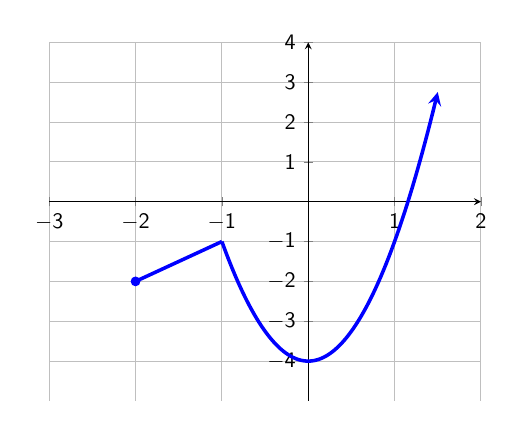
\begin{tikzpicture}[>=stealth, scale=0.8]
    \begin{axis}
    [axis lines = middle, grid,
    xmin = -3, xmax = 2, ymin = -5, ymax = 4,
    % xtick = {-2.5,-2,...,1.5}, 
    ytick = {-4,-3,...,4}
    ]
    \addplot[ultra thick, color=blue,samples=200, domain=-2:-1] {x};
    \addplot[->, ultra thick, color=blue, samples=200, domain=-1:1.5] {3*x^2-4};
    \addplot[color=blue, mark = *] coordinates {(-2,-2)};
    \end{axis}
    \end{tikzpicture}
\end{center}

\begin{multicols}{2}
\begin{enumerate}
\item Domain of $f$
\item Range of $f$
\item Relative Minimum
\item Relative Maximum
\item $f(1)$
\item $f(0)$
\item Increasing Interval(s)
\item Decreasing Interval(s)
\item Absolute Maximum
\item Absolute Minimum
\setcounter{Review}{\value{enumi}}
\end{enumerate}
\end{multicols}

Find each of the following given $f(x) = -2x^{3}+6x^{2}-5x+1$. Round to 3 decimal places and use interval notation when applicable.
\begin{multicols}{2}
\begin{enumerate}
\setcounter{enumi}{\value{Review}}
\item $f(7)$
\item $f(-2)$
\item Rel. Max
\item Rel. Min
\item Global Max
\item Global Min
\item Increasing Interval(s)
\item Decreasing Interval(s)
\end{enumerate}
\end{multicols}

\newpage

\textsc{Properties of Functions Key} 

\section*{Maxima and Minima}

\begin{enumerate}
	\item Rel max @ $(0,5)$; No rel min
	\item Rel max @ $(2.158, 3.248)$; Rel min @ $(-1.158, -4.048)$
	\item Rel Max $(-1.366,10.848)$ and $(1,6)$; \quad Rel Min $(0.366,5.652)$
    \item Rel Max $(-1.716,11.598)$; \quad Rel Min $(1.132,-3.929)$
    \item Rel Max: $(1.095, 12.096)$; \quad Rel Min $(-0.761, -0.680)$
    \item Rel Max: $(1.366, 0.348)$; \quad
    Rel Min: $(-0.366, -4.848)$ and $(2,0)$
	\item About 2.16 hours
\end{enumerate}

\section*{Increasing, Decreasing, and Constant Intervals}

\begin{enumerate}
	\item Increasing: $(-\infty, 0)$ \quad Decreasing: $(0, \infty)$
	\item Increasing: $(-1.158, 2.158)$ \quad Decreasing: $(-\infty, -1.158) \cup (2.158, \infty)$
    \item Inc: $(-\infty,-2) \cup \left(\frac{2}{3},\infty\right)$ \quad Dec: $\left(-2, \frac{2}{3}\right)$
    \item Inc; $(-1,0) \cup (1, \infty)$ \quad Dec: $(-\infty, -1) \cup (0,1)$
    \item Inc: $(-1,\infty)$ \quad No intervals where it is decreasing
    \item Inc: $(-0.761, 1.095)$; \quad Dec: $(-\infty, -0.761) \cup (1.095, \infty)$
    \item Inc: $(-0.366,1.366) \cup (2, \infty)$; \quad
    Dec: $(-\infty, -0.366) \cup (1.366,2)$;
\end{enumerate}

\section*{Miscellaneous}


\begin{enumerate}
    \item $[-2, \infty)$
    \item $[-4, \infty)$
    \item $(0, -4)$
    \item $(-1,-1)$
    \item $-1$
    \item $-4)$
    \item $(-2, -1) \cup (0, \infty)$
    \item $(-1,0)$
    \item $(0,-4)$
    \item None
    \item $-426$
    \item 51
    \item (1.408, 0.272)
    \item $(0.592, \, -0.272)$
    \item None
    \item None
    \item $(0.592, \, 1.408)$
    \item $(-\infty, \, 0.592) \cup (1.408, \, \infty)$
\end{enumerate}
\chapter{Linear Functions and Slope}

\section{Equations of Lines}

Write the equation of each line \textbf{in point-slope form} that goes through each pair of points.
\begin{enumerate}
\item $(-2, 1), \, (7,8)$
\item $(0,4), \, (9,-15)$
\item $(-1,-2), \, (-3,-13)$
\end{enumerate}

\section{Average Rate of Change}

For the function $f(x) = x^2$, compute the average rate of change for each interval.
\begin{enumerate}
\item $[1, 1.1]$
\item $[1, 1.01]$
\item $[1, 1.001]$
\item $[1,1.0001]$
\setcounter{Review}{\value{enumi}}
\end{enumerate}

\begin{enumerate}
\setcounter{enumi}{\value{Review}}
\item For your answers in the previous four problems, what value do your average rates of change get closer and closer to?
\setcounter{Review}{\value{enumi}}
\end{enumerate}

Find the average rate of change of the function $f(x) = -6x^2 + 7x + 4$ over each specified interval.
\begin{enumerate}
\setcounter{enumi}{\value{Review}}
\item $[-2, -1]$
\item $[5, 6]$
\item $[0, 1]$
\item $[5,5.001]$
\item $[5,5.0001]$
\item $[5,5.00001]$
\item What value are your last 3 answers getting closer to?
\setcounter{Review}{\value{enumi}}
\end{enumerate}

For the function $f(x) = -3x^2 + 5$, determine the average rate of change of each over the given interval.
\begin{enumerate}
\setcounter{enumi}{\value{Review}}
    \item $[7, 7.001]$
    \item $[7, 7.0001]$
    \item $[7, 7.00001]$
\setcounter{Review}{\value{enumi}}
\end{enumerate}

\begin{enumerate}
\setcounter{enumi}{\value{Review}}
\item For your answers in the previous three problems, what value do your average rates of change get closer and closer to?
\setcounter{Review}{\value{enumi}}
\end{enumerate}

\newpage

Given $f(x) = \sqrt{x}$, find the average rate of change of each over the given interval.
\begin{enumerate}
\setcounter{enumi}{\value{Review}}
	\item $[1, 1.0001]$
	\item $[1, 1.00001]$
	\item $[1, 1.000001]$
\setcounter{Review}{\value{enumi}}
\end{enumerate}

\begin{enumerate}
\setcounter{enumi}{\value{Review}}
\item For your answers in the previous three problems, what value do your average rates of change get closer and closer to?
\setcounter{Review}{\value{enumi}}
\end{enumerate}


Given $f(x) = 6\sqrt{x}$, find the average rate of change of each over the given interval.
\begin{enumerate}
\setcounter{enumi}{\value{Review}}
	\item $[25,\, 25.1]$
	\item $[25, \, 25.01]$
	\item $[25, \, 25.001]$
\setcounter{Review}{\value{enumi}}
\end{enumerate}

\begin{enumerate}
\setcounter{enumi}{\value{Review}}
\item For your answers in the previous three problems, what value do your average rates of change get closer and closer to?
\setcounter{Review}{\value{enumi}}
\end{enumerate}

Find the average rate of change of the function $f(x) = -7x^3 + 6\sqrt{3x} + 4$ over each interval. Round your answers to 4 decimal places.
\begin{enumerate}	\setcounter{enumi}{\value{Review}}
	\item $[0,1]$
	\item $[10,11]$
	\item $[8,15]$
\end{enumerate}	\setcounter{Review}{\value{enumi}}

\newpage

\section{Answer Key}

\section*{Equations of Lines}
\begin{enumerate}
\item $y-1 = \frac{7}{9}(x+2)$ \text{ or } $y-8=\frac{7}{9}(x-7)$
    \item $y-4 = -\frac{19}{9}(x-0)$ \text{ or } $y+15=-\frac{19}{9}(x-9)$
    \item $y+2 = \frac{11}{2}(x+1)$ \text{ or } $y+13=\frac{11}{2}(x+3)$
\end{enumerate}

\section*{Average Rate of Change}
\begin{multicols}{3}
\begin{enumerate}
\item 2.1
\item 2.01
\item 2.001
\item 2.0001
\item 2
\item 25
\item $-59$
\item 1
\item $-53.006$
\item $-53.0006$
\item $-53.00006$
\item $-53$
\item $-42.003$
\item $-42.0003$
\item $-42.00003$
\item $-42$
\item $-0.499988$
\item $-0.4999988$
\item $-0.49999988$
\item $-0.5$
\item $0.5994$
\item $0.59999$
\item $0.6$
\item $0.6$
\item 3.3923
\item $-2,315.3960$
\item $-2861.4492$
\end{enumerate}
\end{multicols}
\chapter{Function Transformations}

Write the function for $g(x)$ if it is the result of $f(x)$ after the following ordered sequence of transformations.
\begin{enumerate}
\item \begin{enumerate}[(1)]
	\item Vertical stretch by 3
	\item Shift left 1 unit
	\item Reflect across $y$-axis
\end{enumerate}
\item \begin{enumerate}[(1)]
	\item Horizontal compression by 2
	\item Shift up 1 unit
\end{enumerate}
\item \begin{enumerate}[(1)]
	\item Reflect across $x$-axis
	\item Vertical compression by 4
	\item Move right 7 units
\end{enumerate}
\setcounter{Review}{\value{enumi}}
\end{enumerate}

Write the function $g(x)$ that is a result of the following ordered sequence of transformations to $f(x)=|x|$.
\begin{enumerate}
\setcounter{enumi}{\value{Review}}
\item
\begin{enumerate}[(1)]
\item Reflect across $x$-axis
\item Shift right 3 units
\item Horizontal stretch by factor of 5
\end{enumerate}

\item
\begin{enumerate}[(1)]
\item Shift down 2 units
\item Reflect across $y$-axis
\item Shift up 1 unit
\end{enumerate}

\item
\begin{enumerate}[(1)]
\item Horizontal compression by factor of 7
\item Vertical compression by factor of 4
\item Shift left 9 units
\end{enumerate}
\setcounter{Review}{\value{enumi}}
\end{enumerate}

Given $f(x) = \sqrt{x}$, determine the resulting function $g(x)$ after the following ordered sequence of transformations.
\begin{enumerate}
\setcounter{enumi}{\value{Review}}
\item
\begin{enumerate}[(1)]
\item Shift up 2 units
\item Horizontal stretch by 5
\item Shift left 3 units
\end{enumerate}

\item
\begin{enumerate}[(1)]
\item Vertical compression by factor of 3
\item Reflect across $y$-axis
\item Horizontal compression by 5
\end{enumerate}

\item
\begin{enumerate}[(1)]
\item Shift right 8 units
\item Reflect across $x$-axis
\item Horizontal compression by factor of 4
\end{enumerate}
\setcounter{Review}{\value{enumi}}
\end{enumerate}

\newpage

Write the final equation of $g(x)$ if it is found by taking $f(x) = \sqrt{x}$ after the following ordered sequence of transformations.   

\begin{enumerate}	\setcounter{enumi}{\value{Review}}
\item \begin{enumerate}[(1)]
\setlength\itemsep{0pt}
    \item Shift right 2 units
    \item Horizontal stretch by factor 3
    \item Shift down 2 units
    \item Reflect across $x$-axis
\end{enumerate}

\item
\begin{enumerate}[(1)]
\setlength\itemsep{0pt}
    \item Horizontal stretch by factor 3
    \item Shift left 1 unit
    \item Shift up 2 units
    \item Reflect across $y$-axis
\end{enumerate}

\item
\begin{enumerate}[(1)]
\setlength\itemsep{0pt}
    \item Vertical stretch by factor 5
    \item Horizontal stretch by factor 2
    \item Shift up 3 units
    \item Reflect across $x$-axis
\end{enumerate}
\setcounter{Review}{\value{enumi}}
\end{enumerate}

Find the equation for $g(x)$ if $g(x)$ is found by performing the following \emph{ordered} sequence of transformations to $f(x)=\frac{1}{x}$.

\begin{enumerate}	\setcounter{enumi}{\value{Review}}
\item \begin{enumerate}[(1)]
\setlength\itemsep{0pt}
	\item Shift left 3 spaces
	\item Reflect across $y$-axis
	\item Shift down 5 spaces
	\item Vertical stretch by factor of 7
\end{enumerate}
\setcounter{Review}{\value{enumi}}
\end{enumerate}

\begin{enumerate}	\setcounter{enumi}{\value{Review}}
\item \begin{enumerate}[(1)]
\setlength\itemsep{0pt}
	\item Shift up 3 spaces
	\item Reflect across $x$-axis
	\item Shift right 5 spaces
	\item Horizontal compression by factor of 7
\end{enumerate}
\setcounter{Review}{\value{enumi}}
\end{enumerate}

Given $f(x) = x^3$, determine the equation for $g(x)$ after the following \emph{ordered} sequence of transformations to $f(x)$.
\begin{enumerate}	\setcounter{enumi}{\value{Review}}
\item \begin{enumerate}[(1)]
\setlength\itemsep{0pt}
	\item Vertical stretch by factor of 4
	\item Shift up 3 units
	\item Reflect across $y$-axis
	\item Shift down 5 units
\end{enumerate}
\setcounter{Review}{\value{enumi}}
\end{enumerate}

\begin{enumerate}	\setcounter{enumi}{\value{Review}}
\item \begin{enumerate}[(1)]
\setlength\itemsep{0pt}
	\item Horizontal compression by factor of 3
	\item Shift right 4 units
	\item Shift up 1 unit
\end{enumerate}
\setcounter{Review}{\value{enumi}}
\end{enumerate}

\begin{enumerate}	\setcounter{enumi}{\value{Review}}
\item \begin{enumerate}[(1)]
\setlength\itemsep{0pt}
	\item Reflect across $x$-axis
	\item Shift down 5 units
	\item Vertical compression by factor of 5
	\item Horizontal stretch by factor of 9
\end{enumerate}
\setcounter{Review}{\value{enumi}}
\end{enumerate}

Given the graph of $f(x)$ below, find the new coordinates of each point after the following transformations.
\begin{center}
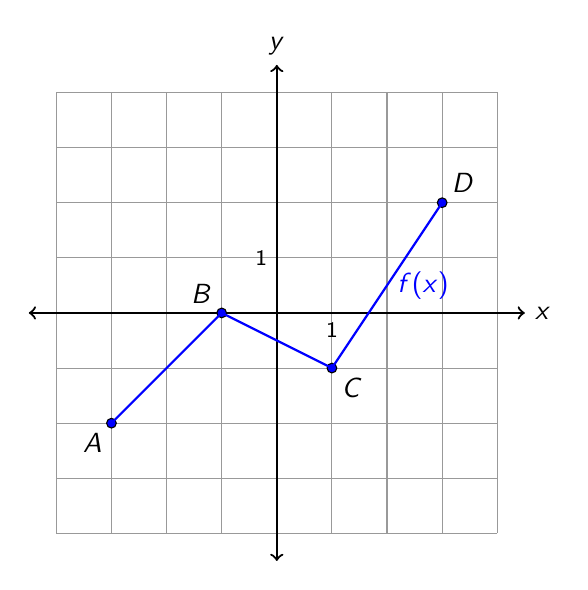
\begin{tikzpicture}[scale=0.7]
\draw[gray!80] (-4,-4) grid (4,4);
\draw[<->, thick] (-4.5,0) -- (4.5,0) node [right] {$x$};
\draw[<->, thick] (0,-4.5) -- (0,4.5) node [above] {$y$};
\coordinate (A) at (-3,-2);
\coordinate (B) at (-1,0);
\coordinate (C) at (1,-1);
\coordinate (D) at (3,2);
\draw[fill=blue] (A) circle [radius=2.5pt] node [below left] {$A$};
\draw[fill=blue] (B) circle [radius=2.5pt] node [above left] {$B$};
\draw[fill=blue] (C) circle [radius=2.5pt] node [below right] {$C$};
\draw[fill=blue] (D) circle [radius=2.5pt] node [above right] {$D$};
\draw[thick,blue] (A) -- (B) -- (C) -- node [midway, right] {$f(x)$} (D);
\node at (1,0) [below] {\footnotesize 1};
\node at (0,1) [left] {\footnotesize 1};
\end{tikzpicture}
\end{center}

\begin{multicols}{3}
\begin{enumerate} \setcounter{enumi}{\value{Review}}
    \item $-2f(x+1)$ 
    \item $f\left(-\frac{1}{2}x\right)-3$
    \item $\frac{1}{2}f(-x-2)+2$
\end{enumerate}	\setcounter{Review}{\value{enumi}}
\end{multicols}
\begin{multicols}{3}
\begin{enumerate}	\setcounter{enumi}{\value{Review}} 
    \item $f(2x+2)-1$
    \item $-3f(-x+1)+2$
    \item $5f\left(-\frac{1}{2}x\right)$
\setcounter{Review}{\value{enumi}}
\end{enumerate}
\end{multicols}

Given $f(x)$ below, determine the coordinates of $A'$, $B'$, $C'$, and $D'$ after the final transformations done to $f$.
\begin{center}
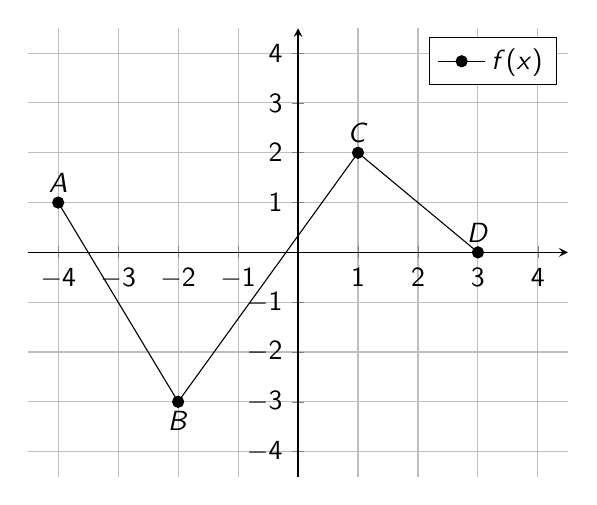
\begin{tikzpicture}
\begin{axis}[
axis lines = middle, xmin = -4.5, xmax = 4.5, xtick distance = 1, ymin = -4.5, ymax = 4.5, ytick distance = 1, grid]
\addplot [mark = *] coordinates {
(-4,1) (-2,-3) (1,2) (3,0)
};
\addlegendentry{$f(x)$};
\node at (-4,1) [above] {$A$};
\node at (-2,-3) [below] {$B$};
\node at (1,2) [above] {$C$};
\node at (3,0) [above] {$D$};
\end{axis}
\end{tikzpicture}
\end{center}
\begin{multicols}{4}
\begin{enumerate}	\setcounter{enumi}{\value{Review}} 
\item $f(-2x-5)+4$
\item $\frac{1}{3}f(x+4)-1$
\item $-3f\left(-\frac{1}{2}x-3\right)$
\item $f(4x+3)+8$
\end{enumerate}	\setcounter{Review}{\value{enumi}}
\end{multicols}



\newpage

\section{Answer Key}

\begin{enumerate}
	\item $g(x) = 3f(-x+1)$
	\item $g(x) = f(2x)+1$
	\item $g(x) = -\frac{1}{4}f(x-7)$
    \item $g(x) = -\left|\frac{1}{5}x-3\right|$
    \item $g(x) = |-x|-1$
    \item $g(x) = \frac{1}{4}|7(x+9)| = \frac{1}{4}|7x+63|$
    \item $g(x) = \sqrt{\frac{1}{5}(x+3)} + 2 = \sqrt{\frac{1}{5}x + \frac{3}{5}}+2$
    \item $g(x) = \frac{1}{3}\sqrt{-5x}$
    \item $g(x) = -\sqrt{4x-8}$
    \item $g(x) = -\left(\sqrt{\frac{1}{3}x-2}-2\right) = -\sqrt{\frac{1}{3}x-2}+2$
    \item $g(x) = \sqrt{\frac{1}{3}(-x+1)}+2 = \sqrt{-\frac{1}{3}x+\frac{1}{3}}+2$
    \item $g(x) = -\left(5\sqrt{\frac{1}{2}x}+3\right) = -5\sqrt{\frac{1}{2}x} - 3$
    \item $g(x) = \frac{7}{-x+3} - 35$
    \item $g(x) = -\frac{1}{7x-5} - 3$ 
    \item $g(x) = 4(-x)^3 - 2$
    \item $g(x) = \left(3(x-4)\right)^3 + 1$
    \item $g(x) = \frac{1}{5}\left(-\frac{1}{9}x\right)^3 - 5$
    \item $A'(-4,4), \, B'(-2,0), \, C'(0,2), \, D'(2,-4)$
    \item $A'(6,-5), \, B'(2,-3), \, C'(-2, -4), \, D'(-6,-1)$
    \item $A'(1,1), \, B'(-1,2), \, C'(-3,1.5), \, D'(-5,3)$
    \item $A'(-2.5,-3), \, B'(-1.5,-1), \, C'(-0.5,-2), \, D'(0.5,1)$
    \item $A'(4,8), \, B'(2,2), \, C'(0,5), \, D'(-2,-4)$
    \item $A'(6,-10), \, B'(2,0), \, C'(-2,-5), \, D'(-6,10)$
    \item $A'\left(-\frac{1}{2},5\right), \, B'\left(-\frac{3}{2},1\right), \, C'(-3,6), \, D'(-4,4)$
	\item $A'\left(-8,-\frac{2}{3}\right), \, B'(-6,-2), \, C'\left(-3,-\frac{1}{3}\right), \, D'(-1,-1)$
	\item $A'(2,-3), \, B'(-2,9), \, C'(-8,-6), \, D'(-12,0)$
	\item $A'\left(-\frac{7}{4},9\right), \, B'\left(-\frac{5}{4},5\right), \, C'\left(-\frac{1}{2},10\right), \, D'(0,8)$
\end{enumerate}

\chapter{Function Operations}

\section{Adding, Subtracting, Multiplying, and Dividing Functions}

Given $f(x) = x + 5$, $g(x) = x^2 - 1$, and $h(x) = \sqrt{x-10}$, simplify or evaluate each.
\begin{enumerate}
    \item $(g-f)(x)$
    \item $(fh)(14)$
    \item $(f+g)(x)$
\setcounter{Review}{\value{enumi}}
\end{enumerate}

Find each of the following given the table below.
\begin{center}
\begin{tabular}{c|c|c|c|c|c|c|c|c|c}
    $\bm{x}$ & $\bm{-4}$ & $\bm{-3}$ & $\bm{-2}$ & $\bm{-1}$ & \textbf{0} & \textbf{1} & \textbf{2} & \textbf{3} & \textbf{4} \\ \hline
    $\bm{f(x)}$ & $-3$ & 0 & $-1$ & 3 & 1 & 2 & 4 & $-4$ & $-2$ \\ \hline
    $\bm{g(x)}$ & 3 & $-1$ & 0 & 1 & 4 & $-2$ & $-4$ & 2 & $-3$ \\
\end{tabular}
\end{center}

\begin{multicols}{5}
\begin{enumerate}	\setcounter{enumi}{\value{Review}}
	\item $(f + g)(-2)$
	\item $(f - g)(0)$
	\item $(fg)(1)$
	\item $\left(\frac{f}{g}\right)(3)$
	\item $(f + f)(-4)$
\setcounter{Review}{\value{enumi}}
\end{enumerate}
\end{multicols}

Find each of the following given the graphs of $f(x)$ (in red) and $g(x)$ (in blue) below:    \newline\\

\begin{center}
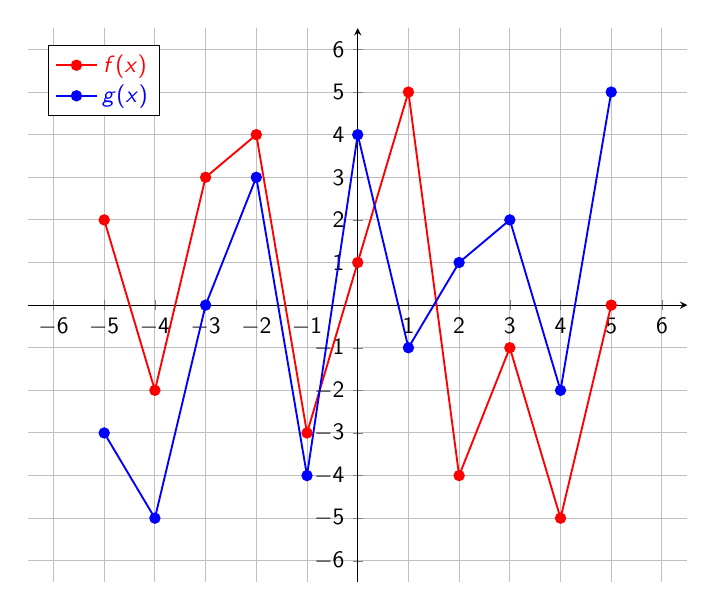
\begin{tikzpicture}[scale=0.85]
\begin{axis}
[xmin=-6.5, xmax=6.5, ymin=-6.5, ymax=6.5, xtick distance = 1, ytick distance = 1, axis lines=center, grid, width=4.5in, legend pos={north west}]
\addplot[color=red, mark=*, thick] coordinates {
(-5, 2) (-4,-2) (-3,3) (-2,4) (-1,-3) (0,1) (1,5) (2,-4) (3,-1) (4,-5) (5,0)
};
\addplot[color=blue, mark=*, thick] coordinates {
(-5, -3) (-4,-5) (-3,0) (-2,3) (-1,-4) (0,4) (1,-1) (2,1) (3,2) (4,-2) (5,5)
};
\addlegendentry{{\color{red}$f(x)$}};
\addlegendentry{{\color{blue}$g(x)$}};
\end{axis}
\end{tikzpicture}
\end{center}

\begin{multicols}{5}
\begin{enumerate}   \setcounter{enumi}{\value{Review}}  \setlength{\itemsep}{8pt}
    \item $(f + g)(2)$
    \item $(f - g)(1)$
    \item $(g - f)(-3)$
    \item $(fg)(4)$
    \item $\left(\frac{f}{g}\right)(0)$
\end{enumerate} \setcounter{Review}{\value{enumi}}
\end{multicols}

\section{Operations with Functions: Domain}

Given $f(x)=\sqrt{2x+7}$ and $g(x) = 3x+3$, find the domain of each.
\begin{enumerate}
\item $(f + g)(x)$
\item $\left(\frac{f}{g}\right)(x)$
\item $\left(\frac{g}{f}\right)(x)$
\end{enumerate}


\section{Difference Quotient}

Write the difference quotient for each.
\begin{enumerate}
	\item $f(x) = 2x - 7$
	\item $g(x) = x^2 + 4x$
	\item $h(x) = -1$
	\item $f(x) = \frac{3}{x+2}$
	\item $g(x) = \sqrt{3x}$
	\item $f(x) = x^2 - 2x + 5$
	\item $g(x) = \frac{5}{x}$
	\item $f(x) = -2x^2 + 3x - 5$
	\item $g(x) = \frac{6}{2x+3}$
	\item $h(x) = \sqrt{7x+5}$
	\item $f(x) = -x^2 + x$
	\item $f(x) = 3x - 1$
	\item $f(x) = x^3 + 5x$
\end{enumerate}


\newpage


\textsc{Function Operations Key}

\section*{Adding, Subtracting, Multiplying, and Dividing Functions}

\begin{enumerate}
    \item $x^2-x-6$
    \item 38
    \item $x^2+x+4$
    \item $-1$
     \item $-3$
     \item $-4$
     \item $-2$
     \item $-6$
     \item $-3$
    \item 6
    \item $-3$
    \item 10
    \item $\frac{1}{4}$
\end{enumerate}

\section*{Operations with Functions: Domain}
\begin{enumerate}
	\item $\left[-\frac{7}{2}, \infty\right)$
    \item $\left[-\frac{7}{2}, -1\right) \cup (-1, \infty)$
    \item $\left(-\frac{7}{2}, \infty\right)$
\end{enumerate}

\section*{Difference Quotient}

\begin{enumerate}
	\item 2
	\item $2x + h + 4$
	\item 0
    \item $\frac{-3}{(x+2)(x+h+2)}$
    \item $\frac{3}{\sqrt{3x+3h}+\sqrt{3x}}$
    \item $2x+h-2$
    \item $\frac{-5}{x(x+h)}$
    \item $-4x-2h+3$
    \item $\frac{-12}{(2x+3)(2x+2h+3)}$
    \item $\frac{7}{\sqrt{7x+7h+5}+\sqrt{7x+5}}$
    \item $-2x - h + 1$
    \item 3
    \item $3x^2 + 3xh + h^2 + 5$
\end{enumerate}
\chapter{Polynomials and Their Graphs}
\everymath{\displaystyle}

Determine the end behavior of each.
\begin{enumerate}
\item $f(x) = -x^5 + \sqrt{7}x^3 - 2x^2$
\item $g(x) = 4x^2 - 16x^6 + 3x$
\item $h(x) = 1 + x^{11} - 4x^8$
\item $f(x) = -x^4+3x^2-2x+6$
\item $g(x) = 0.25x^5-0.1x^4+2x^2-6x$
\item $f(x) = -6x^3 + 2x^2 + 7x^4 - 1$
\item $g(x) = \frac{1}{3}x^3 - \frac{\pi}{8}x^2 + x\sqrt{2} - 3^4$
\end{enumerate}

\newpage

\section{Answer Key}

\begin{enumerate}
	\item $\lim_{x \to -\infty} f(x) = \infty \quad \lim_{x \to \infty}f(x) = -\infty$
	\item $\lim_{x \to -\infty} g(x) = -\infty, \quad \lim_{x \to \infty}g(x) = \infty$
	\item $\lim_{x \to -\infty} h(x) = -\infty \quad \lim_{x \to \infty}h(x) =\infty$
	\item $\lim_{x \to -\infty}f(x) = -\infty$ \quad $\lim_{x \to \infty}f(x) = -\infty$
    \item $\lim_{x \to -\infty}g(x) = -\infty$ \quad $\lim_{x \to \infty}g(x) = \infty$
    \item $\lim_{x \to -\infty} f(x) = \infty \quad \lim_{x \to \infty} f(x) = - \infty$
    \item $\lim_{x \to -\infty} g(x) = -\infty \quad \lim_{x \to \infty} g(x) = \infty$
\end{enumerate}
\chapter{Dividing Polynomials}

\section{Dividing Polynomials}

Divide each.
\begin{enumerate}
    \item $(28x^3-26x^2+41x-15) \div (7x-3)$
    \item $(44y^2+12y^3+61y-37) \div (3y+5)$
    \item $\left(4x^3 - 3x^2 + x + 1\right) \div (x + 2)$
    \item $\left(5x^4 - x^2 + x - 2\right) \div (x^2 + 2)$
    \item $\left(10x^3 + 27x^2 + 8x - 11\right) \div (2x+3)$
	\item $\left(7x^3 + 23x^2 + 12x + 1\right) \div \left(x^2+3x+1\right)$
	\item $\left(28x^3-27x^2-4x+17\right) \div (4x+3)$
	\item $\left(7x^3-27x+4\right) \div \left(x^2-5\right)$
	\item $\left(11x^6-24x^5+15x^4-19x^3-16x^2+21x-8\right) \div (x-2)$
	\item $\left(12x^5-15x^4-11x^3+16x^2-15x+17\right) \div \left(3x^2-5\right)$
	\item $\left(6x^4+20x^3-13x^2+20x+25\right) \div (x+4)$
	\item $\left(24x^5+30x^4-21x^3-4x^2+3x-25\right) \div \left(6x^3+3x^2+3\right)$
	\item $\left(3x^5-22x^4+12x^3+10x^2-7x+24\right) \div \left(3x^2-x-4\right)$
	\item $\left(3x^4-23x^2-15x^3+28x+24\right) \div (x-6)$
	\item $\left(-29x^2+6x^6-29x^3+25x^4-15x^5-25-29x\right) \div \left(3x^3-6x^2-3-x\right)$
	\item $\left(12x^6+16x^5-5x^4+12x^3-17x^2-x-23\right) \div (x+2)$
\end{enumerate}

\section{Remainder and Factor Theorems}

Determine the remainder of each.
\begin{enumerate}
	\item $\left(2x^{53} - 9x^{44} + 13x^8\right) \div (x - 1)$
	\item $\left(x^{71} + 15x^{58} - 3x^{14} + 2\right) \div (x + 1)$
	\item $\left(x^{23}-5x^{20}+17x^8-5\right) \div (x+2)$
	\item $\left(-7x^{17} + 40x^{15} - 6x^8 + 4x^3\right) \div (x-3)$
\end{enumerate}

\newpage

\section{Answer Key}

\section*{Dividing Polynomials}

\begin{enumerate}
    \item $4x^2-2x+5$
    \item $4y^2+8y+7-\frac{72}{3y+5}$
    \item $4x^2 - 11x + 23 - \frac{45}{x+2}$
    \item $5x^2 - 11 + \frac{x+20}{x^2+2}$
    \item $5x^2 + 6x - 5 + \frac{4}{2x+3}$
    \item $7x + 2 + \frac{-x-1}{x^2+3x+1}$
    \item $7x^2-12x+8-\frac{7}{4x+3}$
    \item $7x+\frac{8x+4}{x^2-5}$
    \item $11x^5-2x^4+11x^3+3x^2-10x+1-\frac{6}{x-2}$
    \item $4x^3-5x^2+3x-3+\frac{2}{3x^2-5}$
    \item $6x^3-4x^2+3x+8-\frac{7}{x+4}$
    \item $4x^2+3x-5+\frac{-x^2-6x-10}{6x^3+3x^2+3}$
    \item $x^3-7x^2+3x-5+\frac{4}{3x^2-x-4}$
    \item $3x^3+3x^2-5x-2+\frac{12}{x-6}$
    \item $2x^3-x^2+7x+6+\frac{11x^2-2x-7}{3x^3-6x^2-3-x}$
    \item $12x^5-8x^4+11x^3-10x^2+3x-7-\frac{9}{x+2}$
\end{enumerate}

\section*{Remainder and Factor Theorems}

\begin{enumerate}
	\item 6
	\item 13
	\item $-13,627,141$
    \item $-330,064,119$
\end{enumerate}
\chapter{Rational Functions and Their Graphs}

Find the domain, coordinates of any holes, and equations of all asymptotes.
\begin{multicols}{2}
\begin{enumerate}
\setlength\itemsep{10pt}
	\item $f(x) = \frac{2x^2+5x-3}{2x^2-15x+7}$
	\item $g(x) = \frac{3x^3+7x^2-20x}{x^2-x-12}$
\end{enumerate} \setcounter{Review}{\value{enumi}}
\end{multicols}
\begin{multicols}{2}
\begin{enumerate}	\setcounter{enumi}{\value{Review}}
	\item $f(x) = \frac{3x}{x+4}$
	\item $g(x) = \frac{x^2+3x+2}{x-1}$
\end{enumerate} \setcounter{Review}{\value{enumi}}
\end{multicols}
\begin{multicols}{2}
\begin{enumerate}	\setcounter{enumi}{\value{Review}}
	\item $h(x) = \frac{x^2+3x-4}{x^3-2x^2+x}$
	\item $f(x) = \frac{2x^3-13x^2+6x+45}{x^2-4x-5}$
\end{enumerate} \setcounter{Review}{\value{enumi}}
\end{multicols}
\begin{multicols}{2}
\begin{enumerate}	\setcounter{enumi}{\value{Review}}
	\item $g(x) = \frac{5x^2-19x-4}{x^3+2x^2-24x}$
	\item $h(x) = \frac{2x^2-x-3}{8x^2+51x+18}$
\end{enumerate} \setcounter{Review}{\value{enumi}}
\end{multicols}
\begin{multicols}{2}
\begin{enumerate}	\setcounter{enumi}{\value{Review}}
	\item $f(x) = \frac{6x^3 - 21x^2 - 51x + 30}{3x^2+7x+2}$
	\item $g(x) = \frac{10x^2-29x-21}{10x^3-33x^2-7x}$
\end{enumerate} \setcounter{Review}{\value{enumi}}
\end{multicols}
\begin{multicols}{2}
\begin{enumerate}	\setcounter{enumi}{\value{Review}}
	\item $f(x) = \frac{x^3+x^2-6x}{3x^2-3x-6}$
	\item $f(x) = \frac{x^2-4x+3}{2x^2+2x-12}$
\end{enumerate} \setcounter{Review}{\value{enumi}}
\end{multicols}
\begin{multicols}{2}
\begin{enumerate}	\setcounter{enumi}{\value{Review}}
	\item $f(x) = \frac{x-4}{-2x^2+4x+16}$
	\item $f(x) = \frac{x^3-2x^2-8x}{x^3-2x^2-3x}$
\end{enumerate} \setcounter{Review}{\value{enumi}}
\end{multicols}
\begin{multicols}{2}
\begin{enumerate}	\setcounter{enumi}{\value{Review}}
	\item $f(x) = \frac{x^2+x-2}{3x^2+3x-18}$
	\item $f(x) = \frac{x^2-3x+2}{4x^2-12x}$
\end{enumerate}	\setcounter{Review}{\value{enumi}}
\end{multicols}
\begin{multicols}{2}
\begin{enumerate}	\setcounter{enumi}{\value{Review}}
	\item $f(x) = \frac{8x^2+26x+15}{2x^2-x-15}$
	\item $g(x) = \frac{x^2-1}{2+2x}$
\end{enumerate}	\setcounter{Review}{\value{enumi}}
\end{multicols}
\begin{multicols}{2}
\begin{enumerate}	\setcounter{enumi}{\value{Review}}
	\item $f(x) = \frac{10x^2 + 28x - 6}{12x^2+45x+27}$
	\item $g(x) = \frac{x-5}{x^2-7x+10}$
\end{enumerate}	\setcounter{Review}{\value{enumi}}
\end{multicols}
\begin{multicols}{2}
\begin{enumerate}	\setcounter{enumi}{\value{Review}}
	\item $h(x) = \frac{2x^3-5x^2-42x}{3x-18}$
\end{enumerate}	\setcounter{Review}{\value{enumi}}
\end{multicols}
\vspace{0.25in}

State the end behavior of each.
\begin{enumerate}	\setcounter{enumi}{\value{Review}}
	\item $k(x) = \frac{5x^3-7x^2+8}{-3x^3+6x-4}$
	\item $m(x) = \frac{2x-1}{3x^2+7x+1}$
\end{enumerate}	\setcounter{Review}{\value{enumi}}

%%%%%%%%%%%%%%%%%%%%%%%%%%%%%%%%%%%%%%%%%%%

Answer each of the following given $h(x) = \frac{6x^3+40x^2-14x}{3x^2+11x-4}$
\begin{enumerate}	\setcounter{enumi}{\value{Review}}
	\item End behavior
	\item Domain of $h$
	\item Equation(s) for any vertical asymptotes
	\item Exact coordinates of any holes
	\item What is the approximate value of $h\!\left(5^{933}\right)$?
\end{enumerate}	\setcounter{Review}{\value{enumi}}

\newpage

\section{Answer Key}

\begin{enumerate}
    \item Domain: $x \neq \frac{1}{2}, \, 7$; V.A.: $x=\frac{1}{2}, \, x=7$; H.A.: $y=1$
    \item Domain: $x \neq -3, \, 4$; V.A.: $x=-3 \, x = 4$; Obl. Asymp: $y = 3x+10$
    \item Domain: $x \neq -4$; V.A.: $x = -4$; H.A.: $y = 3$
    \item Domain: $x \neq 1$; V.A.: $x = 1$; Obl. Asymp: $y = x + 4$
    \item Domain: $x \neq 0, 1$; V.A.: $x = 0$ and $x = 1$; H.A.: $y = 0$ 
    \item Domain: $x \neq -1, 5$; V.A. $x=-1$; Hole @ $\left(5, \frac{13}{3}\right)$; Obl. Asym $y = 2x-5$
    \item Domain: $x \neq -6, 0, 4$; V.A. $x = -6, \, x = 0$; Hole @ $\left(4, \frac{21}{40}\right)$; H.A. $y = 0$
    \item Domain: $x \neq -6, -\frac{3}{8}$; V.A. $x = -6, \, x = -\frac{3}{8}$; H.A. $y = \frac{1}{4}$
    \item Domain: $x \neq -2, \, -\frac{1}{3}$; Hole @ $(-2,-21)$; V.A.: $x = -\frac{1}{3}$; Obl. Asymp: $y = 2x-\frac{35}{3}$
    \item Domain: $x \neq -\frac{1}{5}, \, 0, \, \frac{7}{2}$; Hole @ $\left(\frac{7}{2}, \frac{82}{259}\right)$; V.A. $x = -\frac{1}{5}$ and $x=0$; H.A. $y=0$
    \item Domain: $x \neq -1, \, 2$; V.A. $x = -1$; Hole @ $\left(2, \frac{10}{9}\right)$; Obl. Asymp: $y = \frac{1}{3}x+\frac{2}{3}$
    \item Domain: $x \neq -3, \, 2$; V.A. $x = -3$ and $x = 2$; H.A. $y = \frac{1}{2}$
    \item Domain: $x \neq -2, \, 4$; V.A. $x = 2$; Hole @ $\left(4, -\frac{1}{12}\right)$; H.A. $y = 0$
    \item Domain: $x \neq -1, \, 0, \, 3$; V.A. $x = -1$ and $x = 3$; Hole @ $\left(0, \frac{8}{3}\right)$; H.A. $y = 1$
    \item Domain: $x \neq -3, \, 2$; V.A. $x = -3$ and $x = 2$; H.A. $y = \frac{1}{3}$
    \item Domain: $x \neq 0, \, 3$; V.A. $x = 0$ and $x = 3$; H.A. $y = \frac{1}{4}$
    \item Domain: $x \neq -\frac{5}{2}, 3$; V.A. $x = 3$; Hole @ $\left(-\frac{5}{2}, \frac{14}{11}\right)$; H.A. $y = 4$
    \item Domain: $x \neq -1$; No vertical asymptote; Hole @ $(-1,-1)$; Obl. Asymp: $y = \frac{1}{2}x-\frac{1}{2}$
    \item Domain: $x \neq -3, -\frac{3}{4}$; Vert. Asymp: $x = -\frac{3}{4}$; Hole @ $\left(-3, \frac{32}{27}\right)$; Horiz. Asymp: $y = \frac{5}{6}$
    \item Domain: $x \neq 2, 5$; Vert. Asymp: $x = 2$; Hole @ $\left(5, \frac{1}{3}\right)$; Horiz. Asymp: $y = 0$
    \item Domain: $x \neq 6$; Hole @ $\left(6, 38\right)$; Oblique Asymp: $y = \frac{2}{3}x^2 +\frac{7}{3}x$
    
%%%%% End Behavior %%%%%%%%%
    \item $\displaystyle \lim_{x \to -\infty} k(x) = \infty \quad \lim_{x \to \infty} k(x) = -\frac{5}{3}$
    \item $\displaystyle \lim_{x \to -\infty} m(x) = \infty \quad \lim_{x \to \infty} m(x) = 0$
    
    \item $y = 2x + 6$
    \item $x \neq -4, \frac{1}{3}$
    \item $x = -4$
    \item $\left(\frac{1}{3}, \frac{44}{39}\right)$
    \item $2\left(5^{933}\right) + 6$
\end{enumerate}

\chapter{Polynomial and Rational Inequalities}

\section{Polynomial Inequalities}

Solve each. Write your answers using interval notation.
\begin{enumerate}
\item $6x^3-4x^2-10x \geq 0$
\end{enumerate}

\section{Rational Inequalities}

Solve each. Write your answers using interval notation.
\begin{enumerate}
\setlength\itemsep{10pt}
\item $\frac{3x-4}{x+1}<0$
\item $\frac{x^2+3x+2}{x-7} \leq 0$
\end{enumerate}

\newpage

\textsc{Polynomial and Rational Inequalities Key}

\section*{Polynomial Inequalities}
\begin{enumerate}
    \item $[-1,0] \cup \left[\frac{5}{3}, \infty\right)$
\end{enumerate}
\section*{Rational Inequalities}
\begin{enumerate}
    \item $\left(-1, \frac{4}{3}\right)$
    \item $(-\infty,-2] \cup [-1, 7)$
\end{enumerate}
\chapter{Function Compositions}

Given $f(x) = x - 5$, $g(x) = 4 + \sqrt{2x+1}$, and $h(x) = \dfrac{3}{x+7}$, simplify each \underline{and state the domain}.
\begin{enumerate}
	\item $(f \circ g)(x)$
	\item $(g \circ f)(x)$
	\item $h(h(x))$
\setcounter{Review}{\value{enumi}}
\end{enumerate}

Find each of the following given the table below.
\begin{center}
\begin{tabular}{c|c|c|c|c|c|c|c|c|c}
    $\bm{x}$ & $\bm{-4}$ & $\bm{-3}$ & $\bm{-2}$ & $\bm{-1}$ & \textbf{0} & \textbf{1} & \textbf{2} & \textbf{3} & \textbf{4} \\ \hline
    $\bm{f(x)}$ & $-3$ & 0 & $-1$ & 3 & 1 & 2 & 4 & $-4$ & $-2$ \\ \hline
    $\bm{g(x)}$ & 3 & $-1$ & 0 & 1 & 4 & $-2$ & $-4$ & 2 & $-3$ \\
\end{tabular}
\end{center}

\begin{multicols}{5}
\begin{enumerate}	\setcounter{enumi}{\value{Review}}
\item $(f \circ g)(-1)$
\item $(g \circ g)(0)$
\item $(f \circ f)(2)$
\item $(g \circ g)(-3)$
\item $f(g(0))$
\setcounter{Review}{\value{enumi}}
\end{enumerate}
\end{multicols}

Use the table below to answer each.
\begin{center}
    \begin{tabular}{|c|c|c|c|c|c|c|c|c|c|c|}
    \hline 
        $x$ & $-4$ & $-3$ & $-2$ & $-1$ & 0 & 1 & 2 & 3 & 4 \\ \hline 
        $f(x)$ & 1 & $-1$ & $-2$ & 4 & 0 & $-4$ & $-3$ & 3 & 2 \\ \hline 
        $g(x)$ & 0 & $-2$ & 1 & $-4$ & $-3$ & 2 & $-1$ & 4 & 3 \\ \hline 
    \end{tabular}
\end{center}

\begin{multicols}{5}
\begin{enumerate}	\setcounter{enumi}{\value{Review}}
\item $(f \circ g)(-1)$
\item $f(g(3))$
\item $(g \circ f)(0)$
\item $f(f(4))$
\item $g(f(g(1)))$
\setcounter{Review}{\value{enumi}}
\end{enumerate}
\end{multicols}

Given $f(x) = \sqrt{3x+2}$, $g(x) = x^2 - 1$, and $h(x) = 9x-2$, find each of the following.
\begin{enumerate}
\setcounter{enumi}{\value{Review}}
\item $(g \circ f)(x)$
\item $f(g(x))$
\item $(h \circ h)(x)$
\setcounter{Review}{\value{enumi}}
\end{enumerate}

Find each of the following given the graphs of $f(x)$ (in red) and $g(x)$ (in blue) below:    \newline\\

\begin{center}
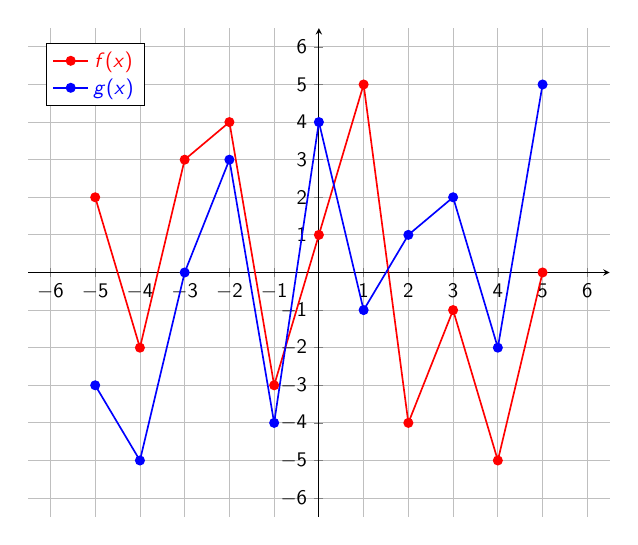
\begin{tikzpicture}[scale=0.75]
\begin{axis}
[xmin=-6.5, xmax=6.5, ymin=-6.5, ymax=6.5, xtick distance = 1, ytick distance = 1, axis lines=center, grid, width=4.5in, legend pos={north west}]
\addplot[color=red, mark=*, thick] coordinates {
(-5, 2) (-4,-2) (-3,3) (-2,4) (-1,-3) (0,1) (1,5) (2,-4) (3,-1) (4,-5) (5,0)
};
\addplot[color=blue, mark=*, thick] coordinates {
(-5, -3) (-4,-5) (-3,0) (-2,3) (-1,-4) (0,4) (1,-1) (2,1) (3,2) (4,-2) (5,5)
};
\addlegendentry{{\color{red}$f(x)$}};
\addlegendentry{{\color{blue}$g(x)$}};
\end{axis}
\end{tikzpicture}
\end{center}

\begin{multicols}{5}
\begin{enumerate}   \setcounter{enumi}{\value{Review}}  
    \item $(f \circ g)(-1)$
    \item $(g \circ f)(-4)$
    \item $f(g(3))$
    \item $g(g(-2))$
    \item $(f \circ f)(-5)$
\end{enumerate} \setcounter{Review}{\value{enumi}}
\end{multicols}

Given $f(x) = \sqrt{2x-9}$ and $g(x) = \frac{2x}{x-3}$, simplify each and state the domain of the composition.

\begin{multicols}{3}
\begin{enumerate}	\setcounter{enumi}{\value{Review}}  
    \item $f(g(x))$
    \item $(g \circ f)(x)$
    \item $g(g(x))$
\end{enumerate}		\setcounter{Review}{\value{enumi}}
\end{multicols}

\newpage

\section{Answer Key}

\begin{enumerate}
	\item $-1 + \sqrt{2x+1}$ Domain: $\left[-\frac{1}{2}, \infty\right)$
	\item $4 + \sqrt{2x-9}$ Domain: $\left[\frac{9}{2}, \infty\right)$
	\item $\frac{3x+21}{7x+52}$ Domain: $\left(-\infty, -\frac{52}{7}\right) \cup \left(-\frac{52}{7}, -7\right) \cup (-7, \infty)$
	\item 2
     \item $-3$
     \item $-2$
     \item 1
     \item $-2$
     \item 1
     \item 2
     \item $-3$
     \item $-3$
     \item $-2$
     \item $3x + 1$
    \item $\sqrt{3x^2-1}$
    \item $81x-20$
    \item $-2$
    \item 3
    \item $-4$
    \item 2
    \item $-4$
    \item $f(g(x)) = \sqrt{\frac{-5x+27}{x-3}}; \quad \left(3, \frac{27}{5}\right]$
    \item $(g \circ f)(x) = \frac{2\sqrt{2x-9}}{\sqrt{2x-9}-3}; \quad \left[\frac{9}{2},9\right) \cup (9, \infty)$
    \item $g(g(x)) = \frac{4x}{9-x}; \quad (-\infty, 3) \cup (3, 9) \cup (9, \infty)$
\end{enumerate}
\chapter{Inverse Functions}

Find the inverse of each. Then state the domain and range of the function and the inverse.

\begin{enumerate}
	\item $f(x) = \sqrt{-2x + 3} + 1$
	\item $g(x) = (x+4)^2 - 1, \, x \leq -4$
	\item $h(x) = \frac{9x}{4x-1}$
\end{enumerate}

\newpage

\textsc{Inverse Functions Key}

\begin{enumerate}
	\item $f^{-1}(x) = -\frac{1}{2}\left((x-1)^2-3\right)$ \newline\\
     \begin{tabular}{c|c|c}
         &   Domain  &   Range   \\  \hline
         $f(x)$ & $(-\infty, 1.5]$ & $[1, \infty)$ \\ \hline
         $f^{-1}(x)$ & $[1, \infty)$ & $(-\infty, 1.5]$ \\ 
     \end{tabular}
     
     \item $g^{-1}(x) = -\sqrt{x+1}-4$   \newline\\
     \begin{tabular}{c|c|c}
         &   Domain  &   Range   \\  \hline
         $g(x)$ & $(-\infty, -4]$ & $[-1, \infty)$ \\ \hline
         $g^{-1}(x)$ & $[-1, \infty)$ & $(-\infty, -4]$ \\ 
     \end{tabular}
     
     \item $h^{-1}(x) = \frac{-x}{9-4x}$ \newline\\
     \begin{tabular}{c|c|c}
         &   Domain  &   Range   \\  \hline
         $h(x)$ & $(-\infty, 1/4) \cup (1/4, \infty) $ & $(\infty, 9/4) \cup (9/4, \infty)$ \\ \hline
         $h^{-1}(x)$ & $(\infty, 9/4) \cup (9/4, \infty)$ & $(-\infty, 1/4) \cup (1/4, \infty) $ \\ 
     \end{tabular}
\end{enumerate}
\chapter{Exponential Functions}

\section{End Behavior}

Determine the end behavior of each. Write your answers using limit notation.
\begin{enumerate}
	\item $f(x) = 3 + e^{2x}$
	\item $h(x) = 5^{-x}$
	\item $h(x) = -\frac{2}{3}e^{x+7} + 1$
\end{enumerate}

\newpage

\textsc{Exponential Functions}

\begin{enumerate}
	\item $\lim_{x \to -\infty} f(x) = 3$ \quad $\lim_{x \to \infty} f(x) = \infty$
	\item $\lim_{x \to -\infty} f(x) = \infty$ \quad $\lim_{x \to \infty} f(x) =0$ 
	\item $\lim_{x \to -\infty} h(x) = 0 \quad \lim_{x \to \infty} h(x) = - \infty$
\end{enumerate}

\chapter{Logarithmic Functions}

Write each of the following in exponential or logarithmic form.
\begin{enumerate}
	\item $\ln(a) = 7$
    \item $\log_4 (x+1) = 9$
    \item $\log (5x) = 30$
    \item $\ln(w) = c$
    \item $5^x = 19$
    \item $8^{-3} = \frac{1}{512}$
    \item $e^{14} = x$
    \item $(1.1)^{-t} = 50$
\end{enumerate}	\setcounter{Review}{\value{enumi}}


Find the domain of each. Write your answers in interval notation.
\begin{enumerate}	\setcounter{enumi}{\value{Review}}
	\item $b(x) = \log_7\left(x^2 - 8x + 6\right)$
	\item $a(x) = \ln\left(\frac{x^2+3x+2}{5x+15}\right)$
	\item $f(x) = -7\ln\left(x^2 + 9x + 8\right)$
	\item $g(x) = \log\left(5x^2 + 13x - 6\right)$
	\item $h(x) = 3\log_2\left(x^3+2x^2-x-2\right)$
	\item $c(x) = \ln\left(4x^2 - 15x - 4\right)$
\end{enumerate}
\setcounter{Review}{\value{enumi}}

State the end behavior of each.
\begin{enumerate}	\setcounter{enumi}{\value{Review}}
	\item $j(x) = 5\log_3\left(2x-5\right) - 2$
\end{enumerate}

\newpage

\textsc{Logarithmic Functions Key}

\begin{enumerate}
	\item $(-\infty, 0.838) \cup (7.162, \infty)$
    \item $(-3, -2) \cup (-1, \infty)$
    \item $(-\infty, -8) \cup (-1, \infty)$
    \item $(-\infty, -3) \cup \left(\frac{2}{5}, \infty\right)$
    \item $(-2, -1) \cup (1, \infty)$
    \item $\left(-\infty, -\frac{1}{4}\right) \cup (4, \infty)$
    \item $\lim_{x \to (5/2)^+} j(x) = -\infty \quad \lim_{x \to \infty} j(x) = \infty$ 
\end{enumerate}

\chapter{Properties of Logarithms}

Expand or condense each completely. Simplify numerical answers.
\begin{multicols}{3}
\begin{enumerate}
	\item $\log_b\left(\frac{x^2}{y^8}\right)$
	\item $\ln\left(ez\right)^3$	\vphantom{$\log_b\left(\frac{x^2}{y^8}\right)$}
	\item $\log_5(x) + \log_5(9) - 2\log_5(w)$	\vphantom{$\log_b\left(\frac{x^2}{y^8}\right)$}
\end{enumerate}	\setcounter{Review}{\value{enumi}}
\end{multicols}
\begin{multicols}{3}
\begin{enumerate}	\setcounter{enumi}{\value{Review}}
	\item $\log_2\left(2^ab^3\right)$	\vphantom{$\ln\left(\frac{w^7}{e^6}\right)$}
	\item $\ln\left(\frac{w^7}{e^6}\right)$
	\item $5\log_4(m) - 3\log_4(n) + 2\log_4(p)$	\vphantom{$\ln\left(\frac{w^7}{e^6}\right)$}
\setcounter{Review}{\value{enumi}}
\end{enumerate}
\end{multicols}
\bigskip

Write an equivalent expression for each of the following using natural logarithms.
\begin{multicols}{6}
\begin{enumerate}
\setcounter{enumi}{\value{Review}}
	\item $\log_7(10)$
	\item $\log_9(x)$
	\item $\log_b(c)$
    \item $\log_3(10)$
    \item $\log_{17}(\pi)$    
    \item $\log_{w}(x)$
\setcounter{Review}{\value{enumi}}
\end{enumerate}
\end{multicols}
\bigskip

Suppose that $\log_a(b) = 5, \, \log_a(c) = 12, \text{ and } \log_a(d) = 9$. Evaluate each of the following.
\begin{multicols}{4}
\begin{enumerate}	\setcounter{enumi}{\value{Review}}
	\item $\log_a(bc)$	\vphantom{$\log_a\left(\frac{d}{c}\right)$}
    \item $\log_a(c^3)$	\vphantom{$\log_a\left(\frac{d}{c}\right)$}
    \item $\log_a\left(\frac{d}{c}\right)$
    \item $\log_a\left(\frac{bd}{c}\right)$
\end{enumerate}	\setcounter{Review}{\value{enumi}}
\end{multicols}
\begin{multicols}{4}
\begin{enumerate}	\setcounter{enumi}{\value{Review}}
    \item $\log_a\left(b^7c\right)$	\vphantom{$\log_a\left(\frac{d}{c}\right)$}
    \item $\log_a\left(\frac{c^2}{d}\right)$
    \item $\log_a\left(\sqrt{bc}\right)$	\vphantom{$\log_a\left(\frac{d}{c}\right)$}
    \item $\log_a\left((bd)^2\right)$	\vphantom{$\log_a\left(\frac{d}{c}\right)$}
\end{enumerate}	\setcounter{Review}{\value{enumi}}
\end{multicols}
\begin{multicols}{4}
\begin{enumerate}	\setcounter{enumi}{\value{Review}}
    \item $\log_a\left(\sqrt[3]{d^2}\right)$	\vphantom{$\log_a\left(\frac{d}{c}\right)$}
    \item $\log_a\left(\sqrt{b^5}\right)$	\vphantom{$\log_a\left(\frac{d}{c}\right)$}
    \item $\log_a\left(\frac{b^6c}{d^3}\right)$
    \item $\log_a\left(b^2c^3d^4\right)$	\vphantom{$\log_a\left(\frac{d}{c}\right)$}
\end{enumerate}
\setcounter{Review}{\value{enumi}}
\end{multicols}

\newpage

\section{Answer Key}

\begin{enumerate}
	\item $2\log_b(x) - 8\log_b(y)$
    \item $3 + 3\ln(z)$
    \item $\log_5\left(\frac{9x}{w^2}\right)$
    \item $a + 3\log_2(b)$
    \item $7\ln(w) - 6$
    \item $\log_4\left(\frac{m^5p^2}{n^3}\right)$
    \item $\frac{\ln(10)}{\ln(7)}$
    \item $\frac{\ln(x)}{\ln(9)}$
    \item $\frac{\ln(c)}{\ln(b)}$
    \item $\frac{\ln(10)}{\ln(3)}$
    \item $\frac{\ln(\pi)}{\ln(17)}$
    \item $\frac{\ln(x)}{\ln(w)}$
    \item 17
    \item 36
    \item $-3$
    \item 2
    \item 47
    \item 15
    \item 17/2
    \item 28
    \item 6
    \item 25/2
    \item 15
    \item 82
\end{enumerate}
\chapter{Exponential Equations}

Solve each. Round to 3 decimal places when necessary.
\begin{multicols}{2}
\begin{enumerate}
	\item $3e^{x-2} = 7$
	\item $5^x + 4 > 1$
\end{enumerate} \setcounter{Review}{\value{enumi}}
\end{multicols}
\begin{multicols}{2}
\begin{enumerate}	\setcounter{enumi}{\value{Review}}
	\item $2^{3x+4} = 32^{x-7}$
	\item $5e^{7x} + 10 = 42$
\end{enumerate} \setcounter{Review}{\value{enumi}}
\end{multicols}
\begin{multicols}{2}
\begin{enumerate}	\setcounter{enumi}{\value{Review}}
	\item $7^{4x+1} \geq 343$
	\item $1000e^{0.04x} = 2000$
\end{enumerate} \setcounter{Review}{\value{enumi}}
\end{multicols}
\begin{multicols}{2}
\begin{enumerate}	\setcounter{enumi}{\value{Review}}
	\item $3(4.1)^{x-2} = 8$
	\item $2^{x+1} = 5^{7x-5}$
\end{enumerate} \setcounter{Review}{\value{enumi}}
\end{multicols}
\begin{multicols}{2}
\begin{enumerate}	\setcounter{enumi}{\value{Review}}
	\item $8(17)^{-5x} = 22$
	\item $-3(11)^{x-10} = -58$
\end{enumerate} \setcounter{Review}{\value{enumi}}
\end{multicols}
\begin{multicols}{2}
\begin{enumerate}	\setcounter{enumi}{\value{Review}}
	\item $12^{-10x}+8=80$
	\item $-5(10)^{7x}+9 = -46$
\end{enumerate} \setcounter{Review}{\value{enumi}}
\end{multicols}
\begin{multicols}{2}
\begin{enumerate}	\setcounter{enumi}{\value{Review}}
	\item $8(8)^{10x}-1 = 55.2$
	\item $3(3)^{-5x}-8=74$
\end{enumerate} \setcounter{Review}{\value{enumi}}
\end{multicols}
\begin{multicols}{2}
\begin{enumerate}	\setcounter{enumi}{\value{Review}}
	\item $6(16)^{4x-9} = 19$
	\item $-7(11)^{5x-7}=-3$
\end{enumerate} \setcounter{Review}{\value{enumi}}
\end{multicols}
\begin{multicols}{2}
\begin{enumerate}	\setcounter{enumi}{\value{Review}}
	\item $3^{9-6x}-7 = 26$
\end{enumerate}
\end{multicols}

\section{Applications}
\begin{enumerate}
	\item Plutonium has a half-life of 24,360 years. If 15 grams are initially present, how long until 9.5 grams remain?
	\item Cadmium-109 has a half-life of about 1.267 years. If 50 mg are initially present, how many years will it take for 16 mg to remain?
    \item The half-life of bismuth-207 is about 32.9 years. If 90 mg are initially present, how many years will it take for 75 mg to remain?
\end{enumerate}

\newpage

\section{Answer Key}

\begin{multicols}{2}
\begin{enumerate}
	\item $x \approx 2.847$
	\item $(-\infty, \infty)$
\end{enumerate} \setcounter{Review}{\value{enumi}}
\end{multicols}
\begin{multicols}{2}
\begin{enumerate}	\setcounter{enumi}{\value{Review}}
	\item $x = 19.5$
	\item $x \approx 0.265$
\end{enumerate} \setcounter{Review}{\value{enumi}}
\end{multicols}
\begin{multicols}{2}
\begin{enumerate}	\setcounter{enumi}{\value{Review}}
	\item $\left[\frac{1}{2}, \infty\right)$
	\item $x \approx 17.329$
\end{enumerate} \setcounter{Review}{\value{enumi}}
\end{multicols}
\begin{multicols}{2}
\begin{enumerate}	\setcounter{enumi}{\value{Review}}
	\item $x \approx 2.695$
    \item $x \approx 0.827$
\end{enumerate} \setcounter{Review}{\value{enumi}}
\end{multicols}
\begin{multicols}{2}
\begin{enumerate}	\setcounter{enumi}{\value{Review}}
    \item $x \approx -0.071$
    \item $x \approx 11.235$
\end{enumerate} \setcounter{Review}{\value{enumi}}
\end{multicols}
\begin{multicols}{2}
\begin{enumerate}	\setcounter{enumi}{\value{Review}}
    \item $x \approx -0.172$
    \item $x \approx 0.149$
\end{enumerate} \setcounter{Review}{\value{enumi}}
\end{multicols}
\begin{multicols}{2}
\begin{enumerate}	\setcounter{enumi}{\value{Review}}
    \item $x \approx 0.094$
    \item $x \approx -0.602$
\end{enumerate} \setcounter{Review}{\value{enumi}}
\end{multicols}
\begin{multicols}{2}
\begin{enumerate}	\setcounter{enumi}{\value{Review}}
    \item $x \approx 2.354$
    \item $x \approx 1.323$
\end{enumerate} \setcounter{Review}{\value{enumi}}
\end{multicols}
\begin{multicols}{2}
\begin{enumerate}	\setcounter{enumi}{\value{Review}}
    \item $x \approx 0.970$
\end{enumerate}
\end{multicols}

\section*{Applications}

\begin{enumerate}
	\item Approximately 17,952 years
	\item Approximately 2.0828 years
    \item Approximately 8.6538 years
\end{enumerate}
\chapter{Logarithmic Equations and Inequalities}

Solve each. Round to 3 decimal places when necessary.
\begin{enumerate}
	\item $\log_5(x) + x\log_5(x) > 0$
	\item $\ln\left(8-x^2\right) = \ln(2-x)$
	\item $\log_{25}\left(\frac{3x+1}{2x-2}\right) = \frac{1}{2}$
	\item $\log_3(2x+1)-\log_3(x-5) = \log_3(x+1)$
	\item $\log_4(x+1) + \log_4(x-5) > 2$
\end{enumerate}

\newpage

\textsc{Logarithmic Equations and Inequalities Key}

\begin{enumerate}
	\item $(1, \infty)$
	\item $x = -2$
	\item $x \approx 1.571$
	\item $x \approx 6.873$
	\item $(1.472, \infty)$
\end{enumerate}
\chapter{Sequences}

Write the first 4 terms of each sequence.
\begin{enumerate}
	\item $a_n = 2(-3)^n$
	\item $b_n = \frac{n!}{2^n}$
	\item $c_{n+1} = 5c_n + 1; \, c_1 = 2$
	\item $d_{n} = \frac{1}{2}d_{n-1} + n; \, d_1 = 3$
\end{enumerate}

\newpage

\textsc{Sequences Key}

\begin{enumerate}
	\item $-6, \, 18, \, -54, \, 162$
    \item $\frac{1}{2}, \, \frac{1}{2}, \, \frac{3}{4}, \, \frac{3}{2}$
    \item 2, 11, 56, 281
    \item $3, \, \frac{7}{2}, \, \frac{19}{4}, \, \frac{51}{8}$
\end{enumerate}
\chapter{Series}

Find the sum of each, if possible.

\begin{enumerate}
    \item $\sum_{i=1}^{\infty} \left(\frac{1}{5}\right)^i$
    \item $\sum_{i=0}^{\infty} 3\left(-\frac{2}{3}\right)^i$
    \item $\sum_{k=1}^{\infty} -2\left(\frac{1}{3}\right)^k$
    \item $\sum_{j=0}^{\infty} -\frac{1}{2}\left(\frac{3}{2}\right)^j$
\setcounter{Review}{\value{enumi}}
\end{enumerate}

Find the sum of each of the following. Round to 4 decimal places when necessary.
\begin{enumerate}   \setcounter{enumi}{\value{Review}}
    \item $9 + 13 + 17 + 21 + \cdots + 1565$
    \item $-3 + 6 - 12 + 24 - 48 + \cdots + 50,331,648$
    \item $1 + \frac{1}{2} + \frac{1}{3} + \frac{1}{4} + \frac{1}{5} + \cdots + \frac{1}{981}$
    \item $2 + 4 + 6 + 8 + 10 + \cdots + 38,214$
\end{enumerate}	\setcounter{Review}{\value{enumi}}

\newpage

\textsc{Series Key}

\begin{enumerate}
	\item $\frac{1}{4}$
    \item $\frac{9}{5}$
    \item $-1$
    \item Diverges
    \item 306,930
    \item $-33,554,433$
    \item $7.4663$
    \item 365,096,556
\end{enumerate}

\appendix
\chapter{Factoring}

Factor each of the following completely.

\begin{multicols}{4}
\begin{enumerate}
\item $x^2 + 2x - 15$
\item $x^2 - 8x + 12$
\item $x^2 + 15x + 56$
\item $5x^2 + 19x - 4$
\item $4x^2 - 5x - 6$
\item $9x^2 - 400$
\item $5x^2-7x-6$
\item $9x^2-54x+45$
\item $3x^3+12x^2+9x$
\item $9y^2-16$
\item $4x^2-28x+49$
\item $14x^2+11xy-15y^2$
\item $6x^2-48x-120$
\item $9x^4-54x^3+45x^2$
\item $16y^2-40y+25$
\item $30x^2+xy-y^2$
\item $8w^2 + 33w + 4$
\item $3p^2+22p-16$
\item $18x^2-27x+4$
\item $14a^2+15a-9$
\item $4x^2-4x-24$
\item $18t^2-9t-5$
\item $6a^2 + 23a + 21$
\item $25x^2-1$
\end{enumerate}
\end{multicols}

\newpage

\textsc{Factoring Key}

\begin{multicols}{4}
\begin{enumerate}
\item $(x + 5)(x-3)$
\item $(x-6)(x-2)$
\item $(x+7)(x+8)$
\item $(5x-1)(x+4)$
\item $(4x+3)(x-2)$
\item $(3x+20)(3x-20)$
\item $(5x+3)(x-2)$
\item $9(x-5)(x-1)$
\item $3x(x+3)(x+1)$
\item $(3y+4)(3y-4)$
\item $(2x-7)^2$
\item $(7x - 5y)(2x + 3y)$
\item $6(x-10)(x+2)$
\item $9x^2(x-1)(x-5)$
\item $(4y-5)^2$
\item $(6x-y)(5x+y)$
\item $(8w+1)(w+4)$
\item $(3p-2)(p+8)$
\item $(6x-1)(3x-4)$
\item $(7a-3)(2a+3)$
\item $4(x-3)(x+2)$
\item $(6t-5)(3t+1)$
\item $(2a+3)(3a+7)$
\item $(5x+1)(5x-1)$
\end{enumerate}
\end{multicols}
\chapter{Complex Fractions}

Simplify each as much as possible.

\begin{multicols}{3}
\begin{enumerate}
\item $\frac{5+\frac{3}{x}}{x-\frac{1}{2}}$
\item $\frac{\frac{1}{x}+\frac{2}{x^2}}{x+\frac{8}{x^2}}$
\item $\frac{3}{2-\frac{x}{x-1}}$
\end{enumerate}	\setcounter{Review}{\value{enumi}}
\end{multicols}
\smallskip
\begin{multicols}{3}
\begin{enumerate}	\setcounter{enumi}{\value{Review}}
\item $\frac{1+\frac{3}{x}}{\frac{2}{x}+7}$
\item $\frac{\frac{4}{x}-\frac{x}{x-2}}{\frac{1}{x}+{\frac{3}{x-2}}}$
\item $\frac{\frac{3}{x+1}-4}{\frac{2}{x+1}}$
\end{enumerate}	\setcounter{Review}{\value{enumi}}
\end{multicols}
\smallskip
\begin{multicols}{3}
\begin{enumerate}	\setcounter{enumi}{\value{Review}}
\item $\frac{\frac{5}{x}+\frac{3}{x-2}}{\frac{7}{x^2-2x}}$
\item $\frac{\frac{1}{x}-\frac{1}{7}}{x-7}$
\item $\frac{\frac{1}{x}+\frac{1}{x+1}}{5}$
\end{enumerate}	\setcounter{Review}{\value{enumi}}
\end{multicols}
\smallskip
\begin{multicols}{3}
\begin{enumerate}	\setcounter{enumi}{\value{Review}}
\item $\frac{\frac{5}{x}-5x}{x-1}$
\item $\frac{\frac{1}{2+x}-\frac{1}{2}}{x}$
\item $\frac{\frac{3}{x-4}+\frac{2x}{x+1}}{4x}$
\end{enumerate}	\setcounter{Review}{\value{enumi}}
\end{multicols}
\smallskip
\begin{multicols}{3}
\begin{enumerate}	\setcounter{enumi}{\value{Review}}
\item $\frac{\frac{1}{x-a}+\frac{1}{a}}{x}$
\item $\dfrac{\frac{1}{x-1}-\frac{1}{x-3}}{\frac{2}{x-1}+\frac{3}{x+1}}$
\item $\dfrac{\frac{2}{x^2-4}+\frac{1}{x-2}}{\frac{4}{x+2}}$
\end{enumerate}
\end{multicols}

\newpage

\section{Answer Key}

\begin{multicols}{3}
\begin{enumerate}
\item $\frac{2(5x+3)}{x(2x-1)}$
\item $\frac{1}{x^2-2x+4}$
\item $\frac{3(x-1)}{x-2}$
\end{enumerate}	\setcounter{Review}{\value{enumi}}
\end{multicols}
\smallskip
\begin{multicols}{3}
\begin{enumerate}	\setcounter{enumi}{\value{Review}}
\item $\frac{x+3}{2+7x}$
\item $\frac{-1(x^2-4x+8)}{2(2x-1)}$
\item $\frac{-4x-1}{2}$
\end{enumerate}	\setcounter{Review}{\value{enumi}}
\end{multicols}
\smallskip
\begin{multicols}{3}
\begin{enumerate}	\setcounter{enumi}{\value{Review}}
\item $\frac{8x-10}{7}$
\item $-\frac{1}{7x}$
\item $\frac{2x+1}{5x(x+1)}$
\end{enumerate}	\setcounter{Review}{\value{enumi}}
\end{multicols}
\smallskip
\begin{multicols}{3}
\begin{enumerate}	\setcounter{enumi}{\value{Review}}
\item $\frac{-5x-5}{x}$
\item $\frac{-1}{2x+4}$
\item $\frac{(x-1)(2x-3)}{4x(x-4)(x+1)}$
\end{enumerate}	\setcounter{Review}{\value{enumi}}
\end{multicols}
\smallskip
\begin{multicols}{3}
\begin{enumerate}	\setcounter{enumi}{\value{Review}}
\item $\frac{1}{a(x-a)}$
\item $\frac{-2x-2}{5x^2-16x+3}$
\item $\frac{x+4}{4x-8}$
\end{enumerate}
\end{multicols}
\end{document}